\chapter{Men�punkt Extras}
\label{Kapitel Extras}

Im Men�punkt ''Extras'' haben Sie diverse Zusatzm�glichkeiten, um die Planung zu erg�nzen und zu �berpr�fen.

\section{Kollision Student}

Dieser Link leitet Sie zu einer Website, auf der Sie Kollisions�berpr�fungen im Stundenplan auf Studentenebene durchf�hren k�nnen. (siehe Abbildung \ref{Kollision_Student})
Sinnvollerweise funktioniert dies erst nach erfolgter Stundenplanung und Zuteilung aller Studenten zu einer Gruppe oder Spezialgruppe.

\begin {figure}
	\centering
	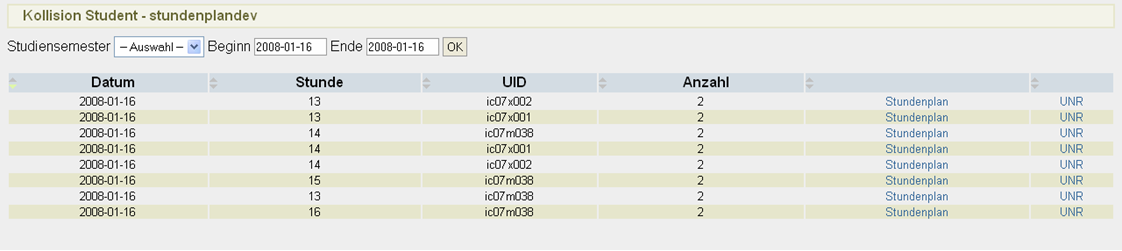
\includegraphics[width=1.0\textwidth]{Tempus_Kollisionscheck_Studenten}
	\caption{Kollisionscheck auf Studentenebene}
	\label{Kollision_Student}
\end {figure}

W�hlen Sie aus den Drop-Down Feldern das gew�nschte Studiensemester und den Zeitraum, zwischen dem �berpr�ft werden soll. Sind Beginn- und Endedatum gleich wird nur jener Tag �berpr�ft.
Wir empfehlen den Zeitraum m�glichst klein zu w�hlen, um die Berechnungszeit zu verk�rzen.

Die daraufhin generierte Liste, wird auf maximal 30 Eintr�ge beschr�nkt.
Sie k�nnen die Liste durch klicken auf die Spalten�berschriften sortieren.

In jeder Zeile finden Sie die Links ''Stundenplan'' und ''UNR'', die jeweils in der unteren Fensterh�lfte Zusatzdetails aufrufen:

Der Link ''Stundenplan'' blendet alle Stunden an diesem Tag in dieser Unterrichtseinheit ein. Mit dem Button ''Delete'' k�nnen Sie danach Eintr�ge l�schen.

Der Link ''UNR'' blendet die Studentenkollision auf Gruppenebene ein.

